%%%%%%%%%%%%%%%%%%%%%%%%%%%%%%%%%%%%%%%%%
% Beamer Presentation
% LaTeX Template
% Version 2.0 (March 8, 2022)
%
% This template originates from:
% https://www.LaTeXTemplates.com
%
% Author:
% Vel (vel@latextemplates.com)
%
% License:
% CC BY-NC-SA 4.0 (https://creativecommons.org/licenses/by-nc-sa/4.0/)
%
%%%%%%%%%%%%%%%%%%%%%%%%%%%%%%%%%%%%%%%%%

%----------------------------------------------------------------------------------------
%	PACKAGES AND OTHER DOCUMENT CONFIGURATIONS
%----------------------------------------------------------------------------------------

\documentclass[
	11pt, % Set the default font size, options include: 8pt, 9pt, 10pt, 11pt, 12pt, 14pt, 17pt, 20pt
	%t, % Uncomment to vertically align all slide content to the top of the slide, rather than the default centered
	%aspectratio=169, % Uncomment to set the aspect ratio to a 16:9 ratio which matches the aspect ratio of 1080p and 4K screens and projectors
]{beamer}

\graphicspath{{Images/}{./}} % Specifies where to look for included images (trailing slash required)

\usepackage{booktabs} % Allows the use of \toprule, \midrule and \bottomrule for better rules in tables

%----------------------------------------------------------------------------------------
%	SELECT LAYOUT THEME
%----------------------------------------------------------------------------------------

% Beamer comes with a number of default layout themes which change the colors and layouts of slides. Below is a list of all themes available, uncomment each in turn to see what they look like.

%\usetheme{default}
%\usetheme{AnnArbor}
%\usetheme{Antibes}
%\usetheme{Bergen}
%\usetheme{Berkeley}
%\usetheme{Berlin}
%\usetheme{Boadilla}
%\usetheme{CambridgeUS}
%\usetheme{Copenhagen}
%\usetheme{Darmstadt}
%\usetheme{Dresden}
%\usetheme{Frankfurt}
%\usetheme{Goettingen}
%\usetheme{Hannover}
%\usetheme{Ilmenau}
%\usetheme{JuanLesPins}
%\usetheme{Luebeck}
\usetheme{Madrid}
%\usetheme{Malmoe}
%\usetheme{Marburg}
%\usetheme{Montpellier}
%\usetheme{PaloAlto}
%\usetheme{Pittsburgh}
%\usetheme{Rochester}
%\usetheme{Singapore}
%\usetheme{Szeged}
%\usetheme{Warsaw}

%----------------------------------------------------------------------------------------
%	SELECT COLOR THEME
%----------------------------------------------------------------------------------------

% Beamer comes with a number of color themes that can be applied to any layout theme to change its colors. Uncomment each of these in turn to see how they change the colors of your selected layout theme.

%\usecolortheme{albatross}
%\usecolortheme{beaver}
%\usecolortheme{beetle}
%\usecolortheme{crane}
%\usecolortheme{dolphin}
%\usecolortheme{dove}
%\usecolortheme{fly}
%\usecolortheme{lily}
%\usecolortheme{monarca}
%\usecolortheme{seagull}
%\usecolortheme{seahorse}
%\usecolortheme{spruce}
%\usecolortheme{whale}
%\usecolortheme{wolverine}

%----------------------------------------------------------------------------------------
%	SELECT FONT THEME & FONTS
%----------------------------------------------------------------------------------------

% Beamer comes with several font themes to easily change the fonts used in various parts of the presentation. Review the comments beside each one to decide if you would like to use it. Note that additional options can be specified for several of these font themes, consult the beamer documentation for more information.

\usefonttheme{default} % Typeset using the default sans serif font
%\usefonttheme{serif} % Typeset using the default serif font (make sure a sans font isn't being set as the default font if you use this option!)
%\usefonttheme{structurebold} % Typeset important structure text (titles, headlines, footlines, sidebar, etc) in bold
%\usefonttheme{structureitalicserif} % Typeset important structure text (titles, headlines, footlines, sidebar, etc) in italic serif
%\usefonttheme{structuresmallcapsserif} % Typeset important structure text (titles, headlines, footlines, sidebar, etc) in small caps serif

%------------------------------------------------

%\usepackage{mathptmx} % Use the Times font for serif text
\usepackage{palatino} % Use the Palatino font for serif text

%\usepackage{helvet} % Use the Helvetica font for sans serif text
\usepackage[default]{opensans} % Use the Open Sans font for sans serif text
%\usepackage[default]{FiraSans} % Use the Fira Sans font for sans serif text
%\usepackage[default]{lato} % Use the Lato font for sans serif text
\usepackage[yyyymmdd]{datetime}


%----------------------------------------------------------------------------------------
%	SELECT INNER THEME
%----------------------------------------------------------------------------------------

% Inner themes change the styling of internal slide elements, for example: bullet points, blocks, bibliography entries, title pages, theorems, etc. Uncomment each theme in turn to see what changes it makes to your presentation.

%\useinnertheme{default}
\useinnertheme{circles}
%\useinnertheme{rectangles}
%\useinnertheme{rounded}
%\useinnertheme{inmargin}

%----------------------------------------------------------------------------------------
%	SELECT OUTER THEME
%----------------------------------------------------------------------------------------

% Outer themes change the overall layout of slides, such as: header and footer lines, sidebars and slide titles. Uncomment each theme in turn to see what changes it makes to your presentation.

%\useoutertheme{default}
%\useoutertheme{infolines}
%\useoutertheme{miniframes}
%\useoutertheme{smoothbars}
%\useoutertheme{sidebar}
%\useoutertheme{split}
%\useoutertheme{shadow}
%\useoutertheme{tree}
%\useoutertheme{smoothtree}

%\setbeamertemplate{footline} % Uncomment this line to remove the footer line in all slides
%\setbeamertemplate{footline}[page number] % Uncomment this line to replace the footer line in all slides with a simple slide count

%\setbeamertemplate{navigation symbols}{} % Uncomment this line to remove the navigation symbols from the bottom of all slides

%----------------------------------------------------------------------------------------
%	PRESENTATION INFORMATION
%----------------------------------------------------------------------------------------

\title[Initation Recherche]{Création de différentes IA en utilisant une architecture I2A} % The short title in the optional parameter appears at the bottom of every slide, the full title in the main parameter is only on the title page

\subtitle{Dans le contexte du jeu Sokoban} % Presentation subtitle, remove this command if a subtitle isn't required

\author[Thomas Guyomard / Jérémy Tremblay]{Thomas Guyomard - Jérémy Tremblay} % Presenter name(s), the optional parameter can contain a shortened version to appear on the bottom of every slide, while the main parameter will appear on the title slide

\institute[]{Université du Littoral Côte d'Opale\\ \smallskip \textit{Encadrant : Jérôme Buisine}} % Your institution, the optional parameter can be used for the institution shorthand and will appear on the bottom of every slide after author names, while the required parameter is used on the title slide and can include your email address or additional information on separate lines

\date[\today]{\today} % Presentation date or conference/meeting name, the optional parameter can contain a shortened version to appear on the bottom of every slide, while the required parameter value is output to the title slide

%----------------------------------------------------------------------------------------

\begin{document}

%----------------------------------------------------------------------------------------
%	TITLE SLIDE
%----------------------------------------------------------------------------------------

\begin{frame}
	\titlepage % Output the title slide, automatically created using the text entered in the PRESENTATION INFORMATION block above
\end{frame}

%----------------------------------------------------------------------------------------
%	TABLE OF CONTENTS SLIDE
%----------------------------------------------------------------------------------------

% The table of contents outputs the sections and subsections that appear in your presentation, specified with the standard \section and \subsection commands. You may either display all sections and subsections on one slide with \tableofcontents, or display each section at a time on subsequent slides with \tableofcontents[pausesections]. The latter is useful if you want to step through each section and mention what you will discuss.

\begin{frame}
	\frametitle{Sommaire} % Slide title, remove this command for no title

	\tableofcontents % Output the table of contents (all sections on one slide)
	%\tableofcontents[pausesections] % Output the table of contents (break sections up across separate slides)
\end{frame}

%----------------------------------------------------------------------------------------
%	PRESENTATION BODY SLIDES
%----------------------------------------------------------------------------------------

 % Sections are added in order to organize your presentation into discrete blocks, all sections and subsections are automatically output to the table of contents as an overview of the talk but NOT output in the presentation as separate slides

%------------------------------------------------


\section{Références}
\begin{frame}
    \frametitle{Références}
    
    \begin{thebibliography}{9}
        
        \bibitem{racaniere2018imagination}
        Sébastien Racanière, Théophane Weber, David P. Reichert, Lars Buesing, Arthur Guez, Danilo Rezende, Adria Puigdomènech Badia, Oriol Vinyals, Nicolas Heess, Yujia Li, Razvan Pascanu, Peter Battaglia, Demis Hassabis, David Silver, Daan Wierstra.
        \newblock Imagination-Augmented Agents for Deep Reinforcement Learning.
        \newblock \textit{DeepMind}, arXiv:1707.06203v2 [cs.LG], 14 Feb 2018.
        
        \bibitem{SchraderSokoban2018}
        Max-Philipp B. Schrader.
        \newblock gym-sokoban.
        \newblock GitHub repository, GitHub, 2018.
        \newblock \url{https://github.com/mpSchrader/gym-sokoban}.
        
    \end{thebibliography}
\end{frame}


%------------------------------------------------
\section{Présentation du jeu Sokoban}

\begin{frame}
	\frametitle{Présentation du jeu Sokoban}

	Jeu de \alert{réflexion}. Le but : le joueur doit ranger des caisses sur des cases cibles.
	\smallskip % Vertical whitespace

	\begin{itemize}
		\item Le personnage a la capacité d'effectuer des déplacement dans chacune des 4 directions possibles. Le niveau est validé une fois toutes les caisses rangées.
	\end{itemize}

	\smallskip % Vertical whitespace

	\begin{figure}
		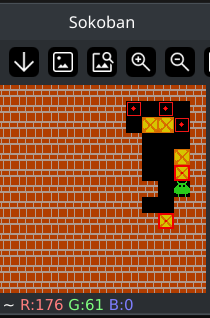
\includegraphics[width=0.2\linewidth]{Images/sokaibanfailed2.png}
		\caption{Capture d'écran du jeu Sokoban.}
	\end{figure}	

\end{frame}

%------------------------------------------------
\section{Agents Augmentés par l'Imagination}

\begin{frame}
	\frametitle{Agents Augmentés par l'Imagination \ / (I2A)}

	\smallskip % Vertical whitespace

	\begin{definition}
	\alert{L'apprentissage par renforcement avec augmentation par l'imagination} appelée \alert{I2A} est une approche du domaine de l'intelligence artificielle permettant d'améliorer la prise de décision des agents d'apprentissage.
	Les agents combinent l'apprentissage automatique avec et sans modèles avec des générations de scénarios pour anticiper des situations inédites et proposer des solutions optimales.
	\end{definition}

	\smallskip % Vertical whitespace

\end{frame}

%------------------------------------------------

\section{IA Q-learning avec une représentation en tableau}

\begin{frame}
	\frametitle{IA Q-learning avec une représentation en tableau}

	\begin{block}{Definitions}
		L'implémentation combine le Q-learning avec un modèle interne I2A pour résoudre le problème complexe du Sokoban, un jeu de réflexion.
	\end{block}

	\smallskip % Vertical whitespace

	\begin{figure}
		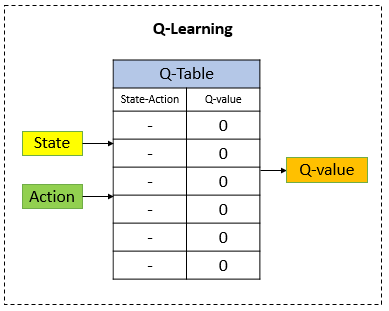
\includegraphics[width=0.5\linewidth]{Images/q_learning.png}
		\caption{Schéma du fonctionnement du Q-Learning.}
	\end{figure}


\end{frame}
%------------------------------------------------
\section{Implémentation du Q-learning}

\begin{frame}
	\frametitle{Implémentation du Q-learning}

	\begin{itemize}
        \item \textbf{Q-table} Contient les états / actions du jeu, elle est initialisée avec des zéros.
        \item \textbf{Boucle d'apprentissage} Itérations sur des épisodes pour mettre à jour la Q-table.
        \item \textbf{Système de récompenses} Intégration des récompenses conformément à la politique définie.
        \item \textbf{Mise à jour de la \textbf \textit Q-table} Prise en compte de la récompense immédiate et de l'estimation de la récompense future.
        \item \textbf{Exploration et Exploitation} Equilibre les connaissances actuelles et permet davantage d'apprentissage.
    \end{itemize}

    \begin{block}{Contenu de la Q-table}
        \textcolor{blue}{\texttt{1146848432601504200: array([-0.05, 2.77913742, 1.69800543, 3.03067097, 2.54018055, 2.77913742, 2.77913742, 3.03067097, 2.54018055])}}
    \end{block}

\end{frame}

%------------------------------------------------
\section{Résultats du Q-learning}

\begin{frame}
    \frametitle{Résultats du Q-learning (1/6)}
    \begin{columns}
        \begin{column}{0.4\textwidth}
            \begin{figure}
                \centering
                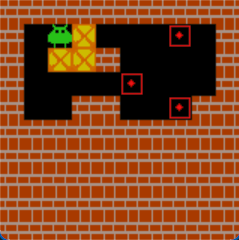
\includegraphics[width=\textwidth]{Images/imagejeux.png}
                \caption{Évolution des récompenses totales obtenues par épisode.}
            \end{figure}
        \end{column}
        \begin{column}{0.4\textwidth}
            \textbf{Contexte de jeu :}\\
            \begin{itemize}
                \item[$\bullet$] Niveau de taille moyenne
                \item[$\bullet$] Jeu de 10x10 cases
                \item[$\bullet$] 3 caisses à pousser
            \end{itemize}
            \vspace{0.5cm}
            \textbf{Contexte d'exécution :}\\
            \begin{itemize}
                \item[$\bullet$] 10 000 parties réalisées
                \item[$\bullet$] Utilisation d'un algorithme de Q-learning 
                \item[$\bullet$] 8h30 de temps d'exécution au total
            \end{itemize}
        \end{column}
    \end{columns}
\end{frame}



\begin{frame}
    \frametitle{Résultats du Q-learning (2/6)}
    \begin{figure}
        \centering
        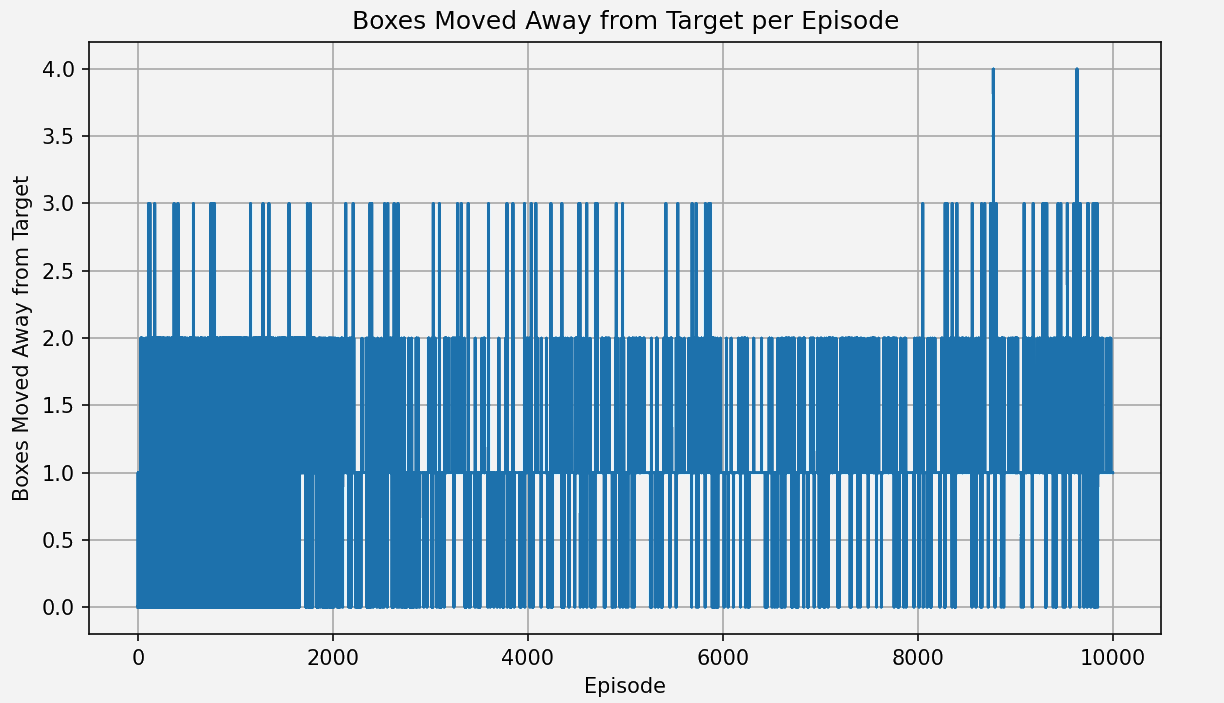
\includegraphics[width=0.7\textwidth]{Images/resultat2.png}
        \caption{Évolution du nombre de caisses poussées en dehors des emplacements par épisode.}
		\begin{block}{Observation des résultats}
			\small L'agent a tendance à pousser une ou deux caisses en dehors des emplacements par épisode.
		\end{block}
    \end{figure}
\end{frame}

\begin{frame}
    \frametitle{Résultats du Q-learning (3/6)}
    \begin{figure}
        \centering
        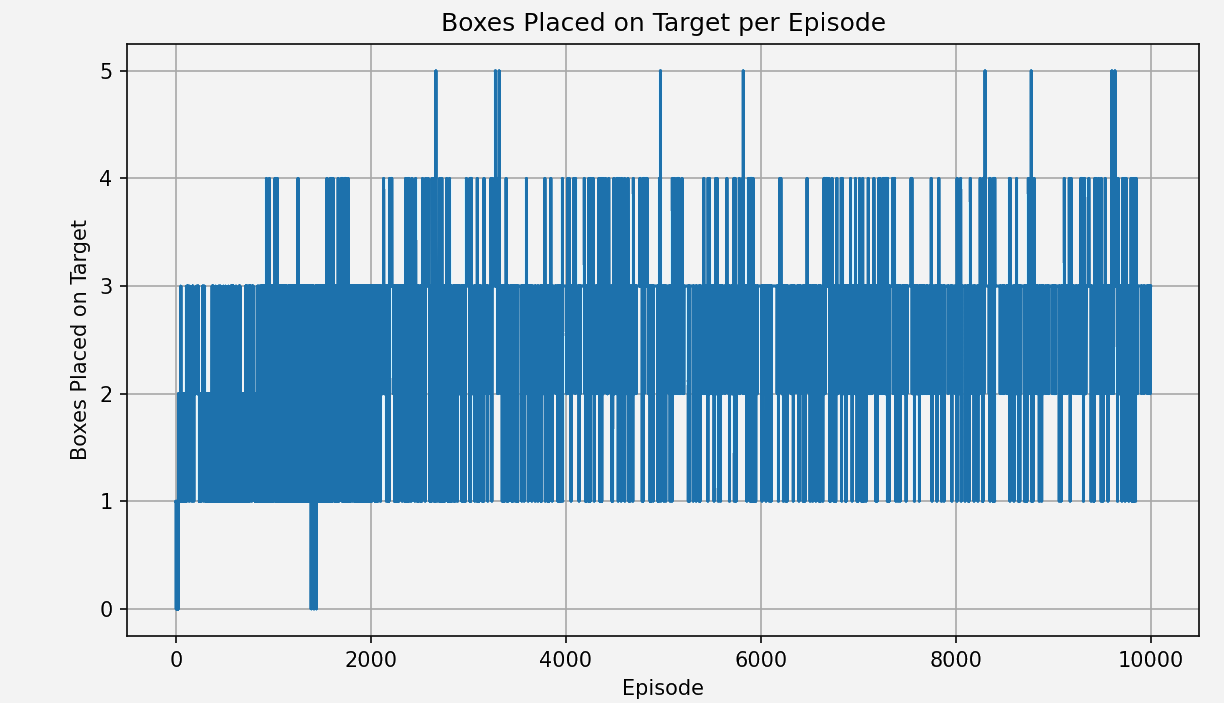
\includegraphics[width=0.75\textwidth]{Images/resultat4.png}
        \caption{Évolution du nombre de caisses poussées sur un emplacement par épisode.}
    \end{figure}
	\begin{block}{Observation des résultats}
        \footnotesize L'agent a compris qu'il devait pousser des caisses sur un emplacement.
    \end{block}
\end{frame}

\begin{frame}
    \frametitle{Résultats du Q-learning (4/6)}
    \begin{figure}
        \centering
        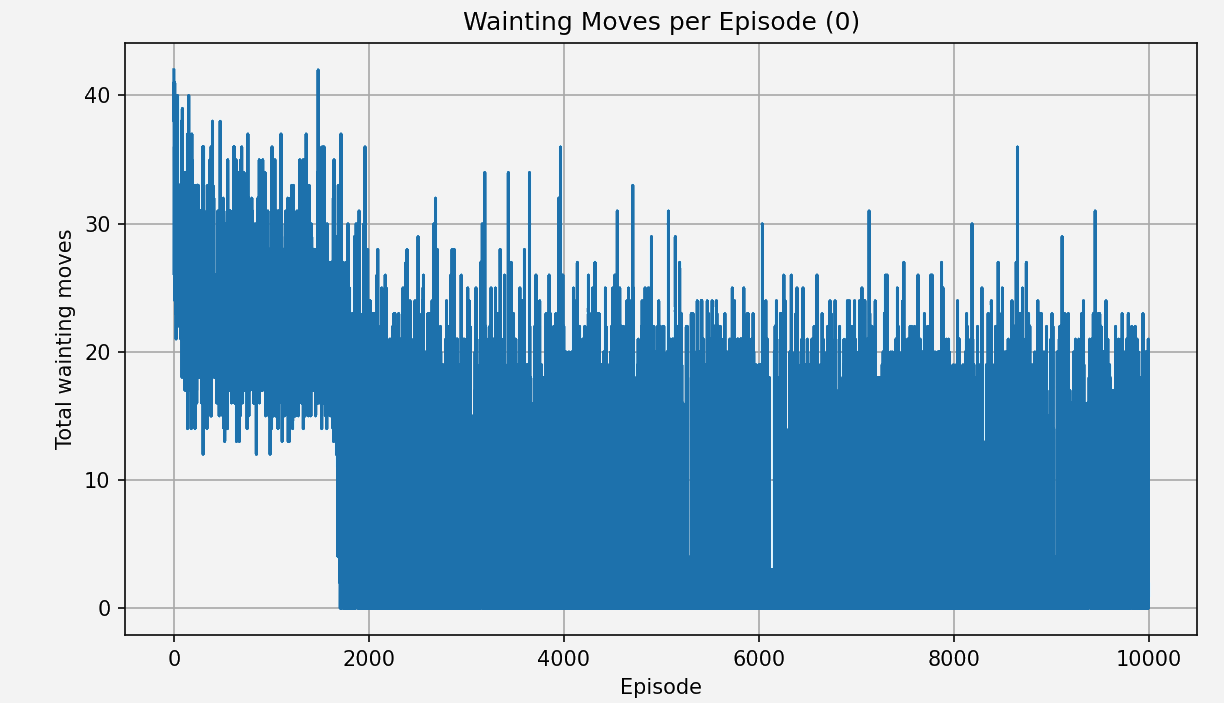
\includegraphics[width=0.8\textwidth]{Images/resultat3.png}
        \caption{Évolution du nombre d'inactions par épisode.}
    \end{figure}
	\begin{block}{Observation des résultats}
        \small L'agent a compris que les mouvements blancs étaient inutiles.
    \end{block}
\end{frame}

\begin{frame}
    \frametitle{Résultats du Q-learning (5/6)}
    \begin{figure}
        \centering
        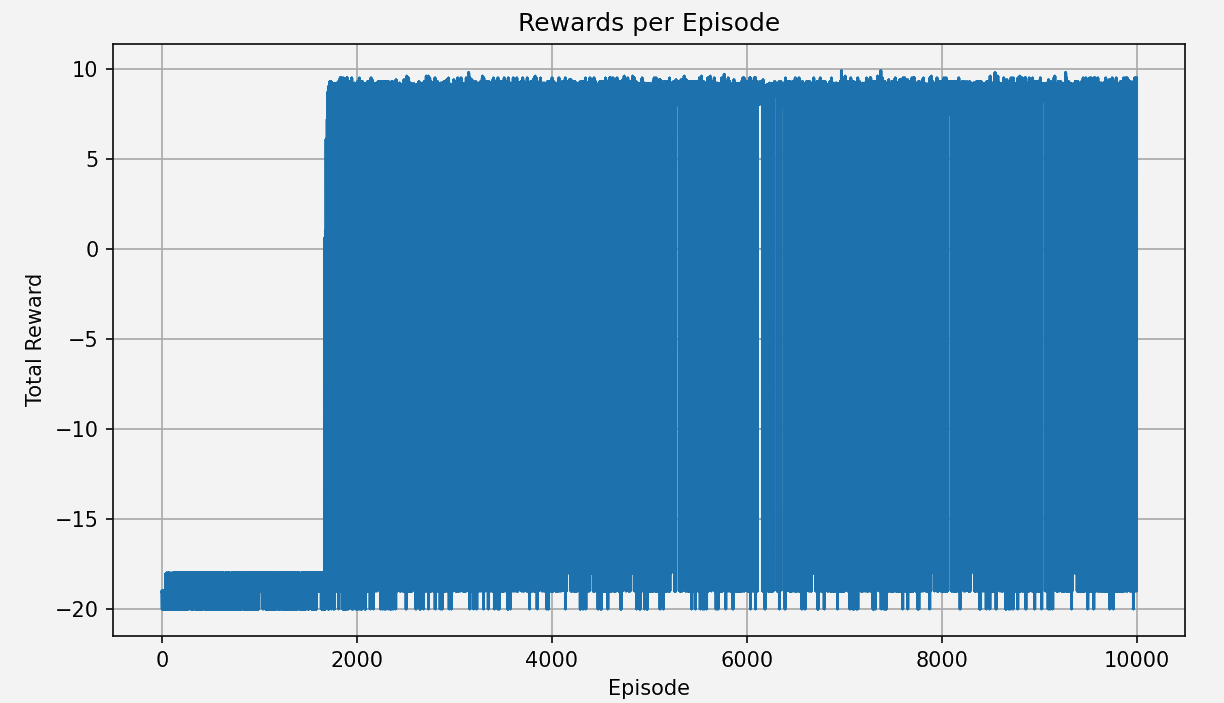
\includegraphics[width=0.8\textwidth]{Images/resultat1.png}
		\caption{Évolution des récompenses totales obtenues par épisode.}
    \end{figure}
	\begin{block}{Observation des résultats}
        \small Changement de comportement : Exploration $\rightarrow$ Exploitation.
    \end{block}

\end{frame}

\begin{frame}
    \frametitle{Résultats du Q-learning (6/6)}
    \begin{figure}
        \centering
        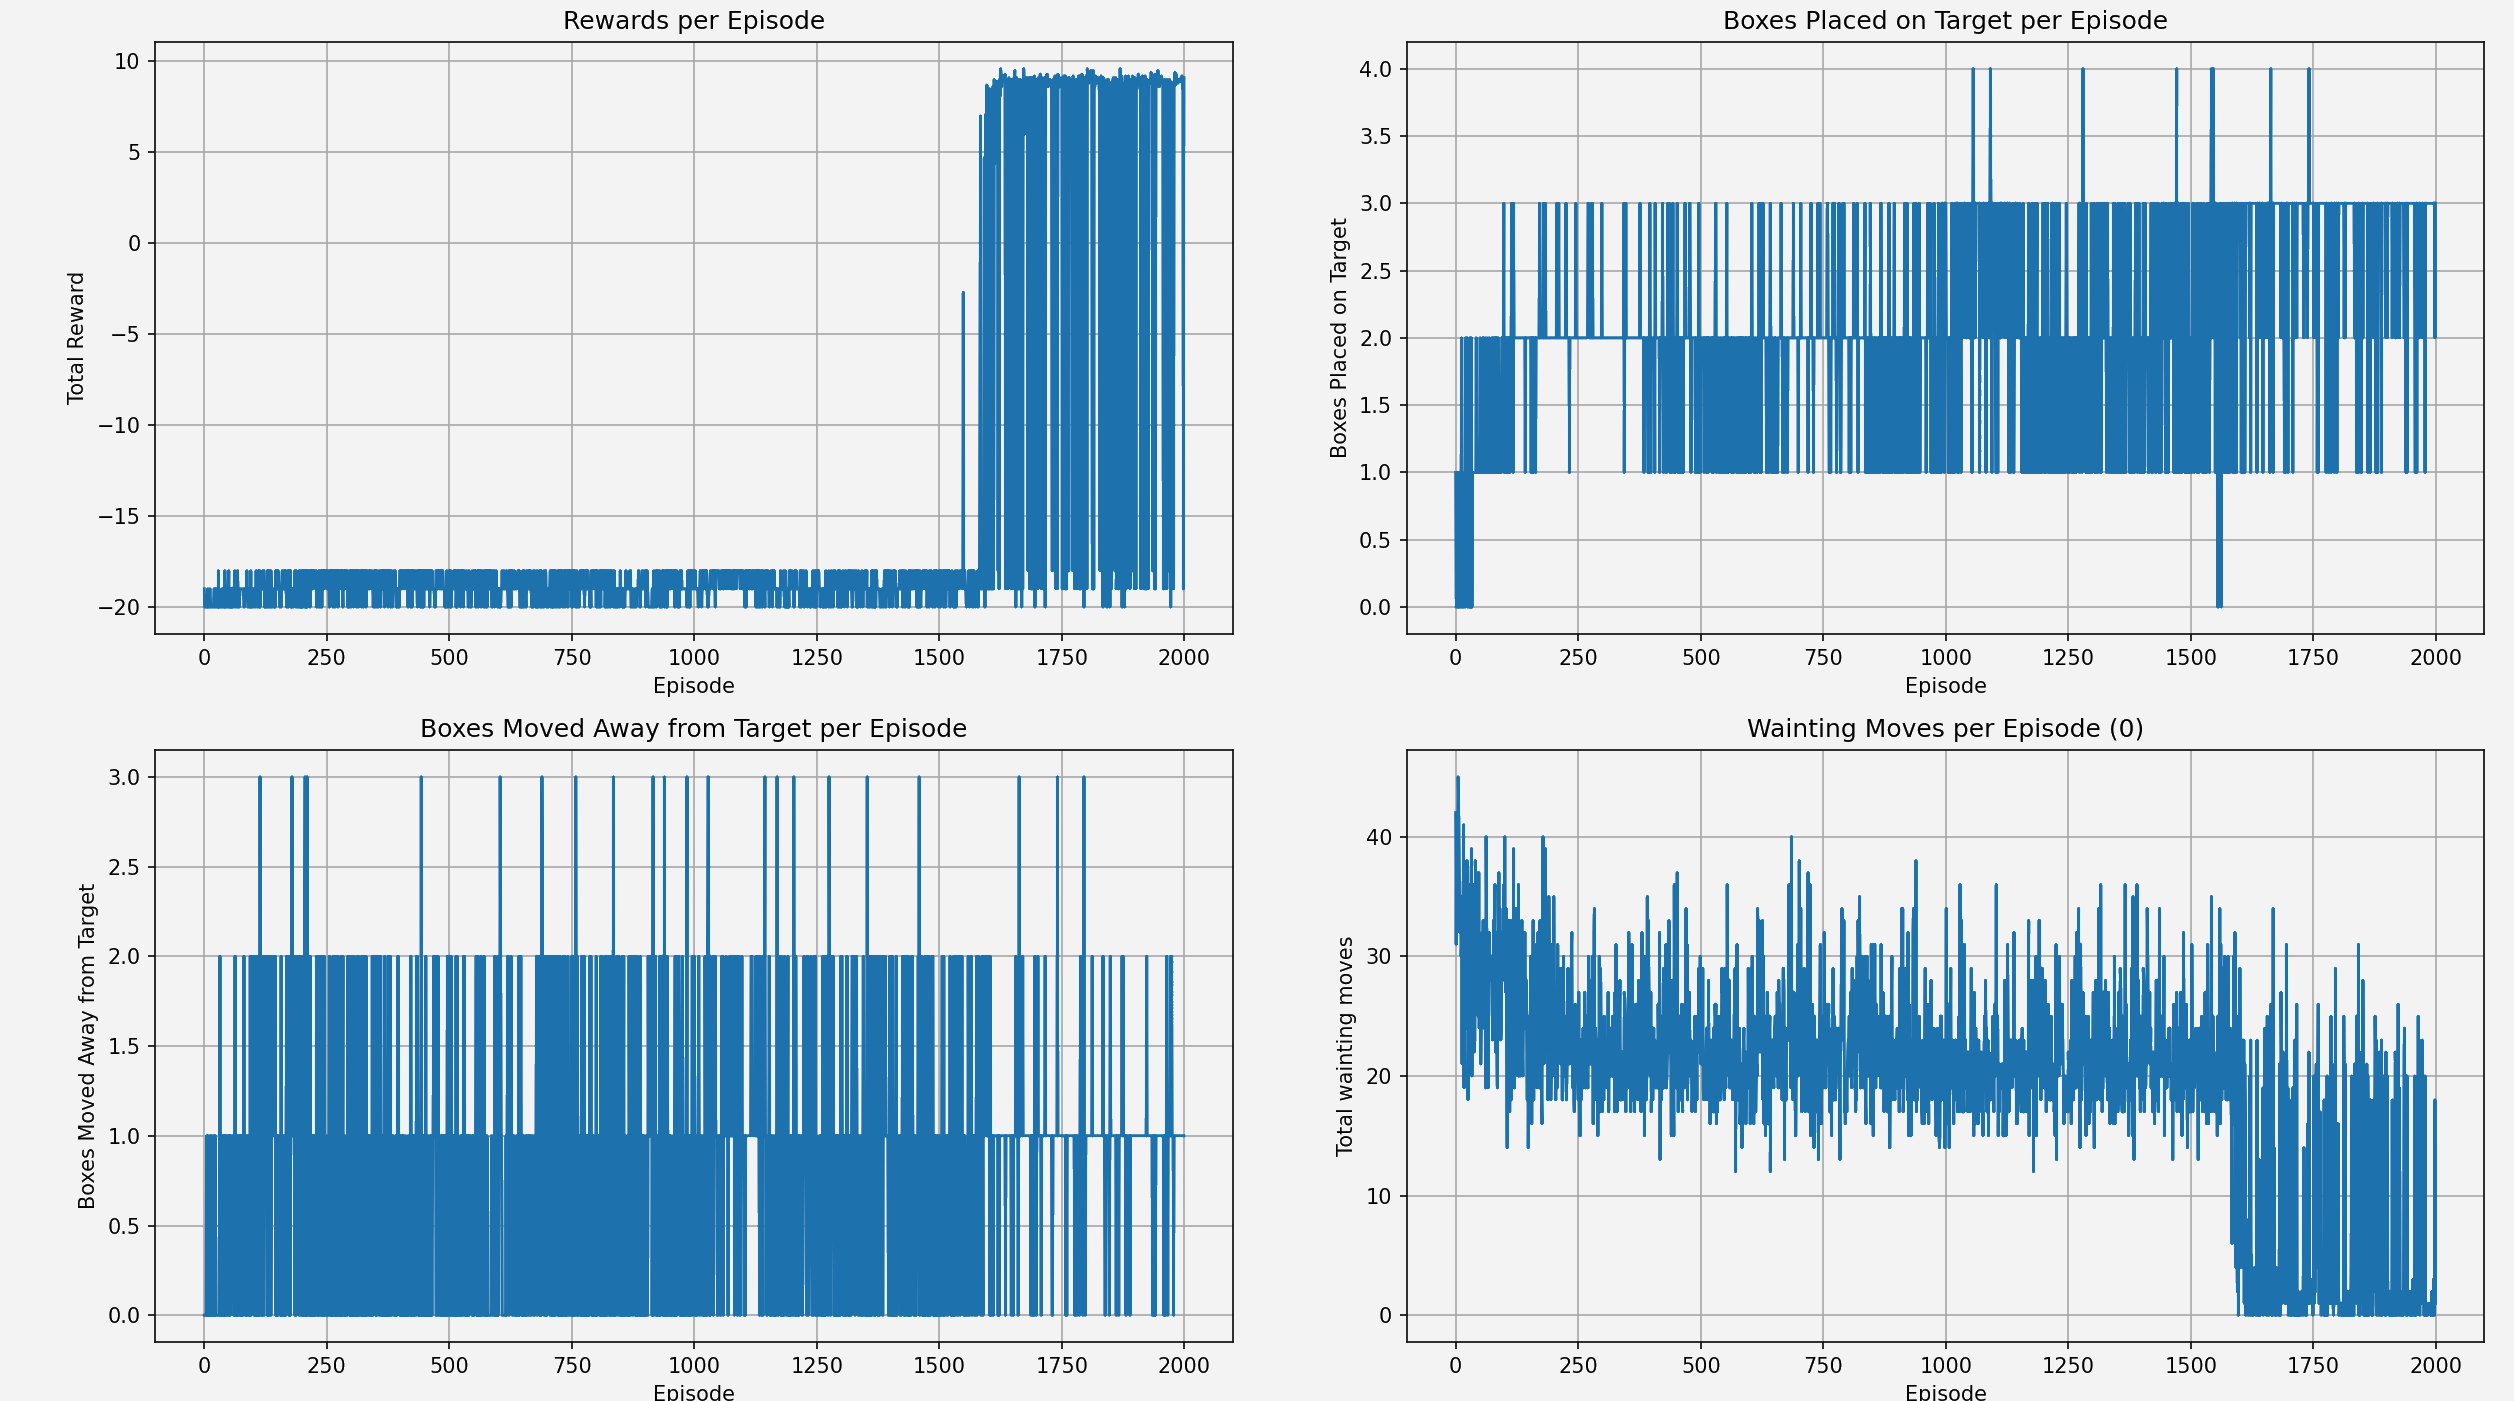
\includegraphics[width=0.9\textwidth]{Images/resultat_2000.png}
		\caption{Résultats du Q-learning sur 2000 épisodes.}
    \end{figure}
\end{frame}


%------------------------------------------------
\section{Plan de Travail}

\begin{frame}{Plan de Travail}
    \begin{table}
        \centering
		\small
        \begin{tabular}{|c|p{8cm}|}
			\hline
            1 & Exploiter notre implémentation du deep Q-learning et comparer les résultats avec ceux du Q-learning.  \\
            \hline
            2 & Finaliser le MCTS et analyser les résultats.  \\
            \hline
            3 & Explorer la possibilité d'utiliser les représentations visuelles de Gym Sokoban pour enrichir la planification. \\
            \hline
            4 & Tester l'agent sur différents niveaux afin d'évaluer sa capacité de généralisation. \\
            \hline
            5 & Si possible, analyser les performances de chaque approche, en mettant en évidence les forces et les faiblesses dans le contexte de Sokoban. \\
            \hline
        \end{tabular}
    \end{table}
\end{frame}

%----------------------------------------------------------------------------------------
%	CLOSING SLIDE
%----------------------------------------------------------------------------------------

\begin{frame}[plain] % The optional argument 'plain' hides the headline and footline
	\begin{center}
		{\Huge Merci pour votre attention.}

	\end{center}
\end{frame}
%----------------------------------------------------------------------------------------

\end{document}
